\chapter{Gretl and Ox}
\label{chap:gretlOx}

\section{Introduction}
\label{Ox-intro}

\app{Ox}, written by Jurgen A. Doornik (see Doornik, 2007), is
described by its author as ``an object-oriented statistical system. At
its core is a powerful matrix language, which is complemented by a
comprehensive statistical library. Among the special features of Ox
are its speed [and] well-designed syntax\dots{}.  Ox comes in two
versions: Ox Professional and Ox Console. Ox is available for Windows,
Linux, Mac (OS X), and several Unix platforms.''
(\url{www.doornik.com})

\app{Ox} is proprietary, closed-source software.  The command-line
version of the program is, however, available free of change for
academic users.  Quoting again from Doornik's website: ``The
Console (command line) versions may be used freely for academic
research and teaching purposes only\dots{}. The Ox syntax is public,
and, of course, you may do with your own Ox code whatever you wish.''
If you wish to use \app{Ox} in conjunction with \app{gretl} please
refer to \url{doornik.com} for further details on licensing.

As the reader will no doubt have noticed, all the other software that
we discuss in this Guide is open-source and freely available for all
users.  We make an exception for \app{Ox} on the grounds that it is
indeed fast and well designed, and that its statistical library ---
along with various add-on packages that are also available --- has
exceptional coverage of cutting-edge techniques in econometrics.  The
\app{gretl} authors have used \app{Ox} for benchmarking some of
\app{gretl}'s more advanced features such as dynamic panel models and
the state space models.\footnote{For a review of \app{Ox}, see
  Cribari-Neto and Zarkos (2003) and for a (somewhat dated) comparison
  of \app{Ox} with other matrix-oriented packages such as \app{GAUSS},
  see Steinhaus (1999).}

\section{\app{Ox} support in \app{gretl}}
\label{sec:Ox-support}

The support offered for \app{Ox} in \app{gretl} is similar to that
offered for \app{R}, as discussed in chapter~\ref{chap:gretlR}, but
with a few differences.  The first difference to note is that 
\app{Ox} support is not on by default; it must be enabled explicitly.

\tip{To enable support for \app{Ox}, go to the
  Tools/Preferences/General menu item and check the box labeled
  ``Enable Ox support''.
  Click ``OK'' in the preferences dialog, then
  quit and restart \app{gretl}.  You will now find, under the Programs
  tab in the Tools/Preferences/General dialog, an entry for specifying
  the path to the \texttt{oxl} executable, that is, the program that
  runs \app{Ox} files (on MS Windows it is called \texttt{oxl.exe}).
  Make sure that path is right, and you're ready to go.}
  
With support enabled, you can open and edit \app{Ox} programs in the
\app{gretl} GUI.  Clicking the ``execute'' icon in the editor window
will send your code to \app{Ox} for execution.
Figures~\ref{fig:Oxedit} and Figure~\ref{fig:Oxout} show an \app{Ox}
program and part of its output.

\begin{figure}[htbp]
  \centering
  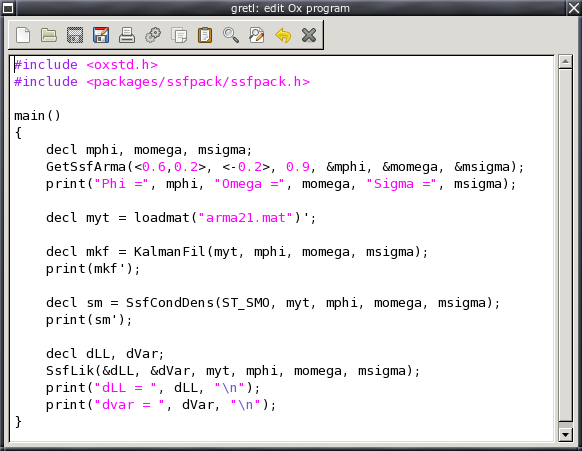
\includegraphics[scale=0.7]{figures/Oxedit}
  \caption{\app{Ox} editing window}
  \label{fig:Oxedit}
\end{figure}

\begin{figure}[htbp]
  \centering
  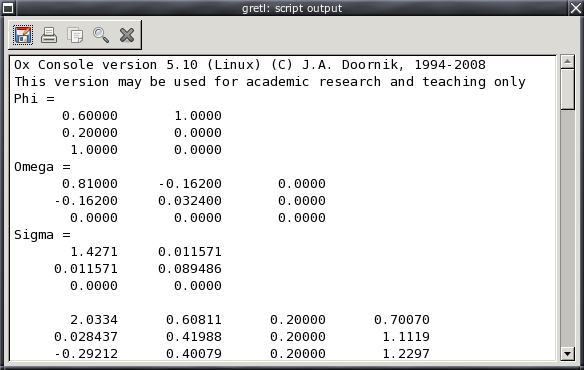
\includegraphics[scale=0.7]{figures/Oxout}
  \caption{Output from \app{Ox}}
  \label{fig:Oxout}
\end{figure}

In addition you can embed \app{Ox} code within a \app{gretl} script
using a \texttt{foreign} block, as described in connection with
\app{R}.  A trivial example, which simply prints the \app{gretl} data
matrix within \app{Ox}, is shown below:
%
\begin{code}
open data4-1
matrix m = { dataset }
mwrite(m, "@dotdir/gretl.mat")

foreign language=Ox 
#include <oxstd.h>
main()
{
   decl gmat = gretl_loadmat("gretl.mat");
   print(gmat);
}
end foreign
\end{code}

The above example illustrates how a matrix can be passed from
\app{gretl} to \app{Ox}.  We use the \texttt{mwrite} function to write
a matrix into the user's ``dotdir'' (see
section~\ref{sec:named-strings}), then in \app{Ox} we use the function
\verb|gretl_loadmat| to retrieve the matrix.

How does \verb|gretl_loadmat| come to be defined?  When \app{gretl}
writes out the \app{Ox} program corresponding to your \texttt{foreign}
block it does two things in addition.  First, it writes a small
utility file named \verb|gretl_io.ox| into your dotdir.  This contains
a definition for \verb|gretl_loadmat| and also for the function
\verb|gretl_export| (see below).  Second, \app{gretl} interpolates
into your \app{Ox} code a line which includes this utility file (it is
inserted right after the inclusion of \texttt{oxstd.h}, which is
needed in all \app{Ox} programs).  Note that \verb|gretl_loadmat|
expects to find the named file in the user's dotdir.

\section{Illustration: replication of DPD model}
\label{sec:dpd-replication}

Example~\ref{Ox-DPD} shows a more ambitious case.  This script
replicates one of the dynamic panel data models in Arellano and Bond
(1991), first using \app{gretl} and then using \app{Ox}; we then check
the relative differences between the parameter estimates produced by
the two programs (which turn out to be reassuringly small).

Unlike the previous example, in this case we pass the dataset from
\app{gretl} to \app{Ox} as a CSV file in order to preserve the
variable names.  Note the use of the internal variable \verb|csv_na|
to get the right representation of missing values for use with
\app{Ox} --- and also note that the \verb|--send-data| option for the
\texttt{foreign} command is not available in connection with Ox.

We get the parameter estimates back from \app{Ox} using
\verb|gretl_export| on the \app{Ox} side and \texttt{mread} on the
\app{gretl} side.  The \verb|gretl_export| function takes two
arguments, a matrix and a file name.  The file is written into the
user's dotdir, from where it can be picked up using \texttt{mread}.
The final portion of the output from Example~\ref{Ox-DPD} is shown
below:
%
\begin{code}
? matrix oxparm = mread("/home/cottrell/.gretl/oxparm.mat")
Generated matrix oxparm
? eval abs((parm - oxparm) ./ oxparm)
  1.4578e-13 
  3.5642e-13 
  5.0672e-15 
  1.6091e-13 
  8.9808e-15 
  2.0450e-14 
  1.0218e-13 
  2.1048e-13 
  9.5898e-15 
  1.8658e-14 
  2.1852e-14 
  2.9451e-13 
  1.9398e-13 
\end{code}

\begin{script}[htbp]
  \caption{Estimation of dynamic panel data model via \app{gretl} and \app{Ox}}
\begin{scode}
open abdata.gdt

# Take first differences of the independent variables
genr Dw = diff(w)
genr Dk = diff(k)
genr Dys = diff(ys)

# 1-step GMM estimation
arbond 2 ; n Dw Dw(-1) Dk Dys Dys(-1) 0 --time-dummies
matrix parm = $coeff

# Write CSV file for Ox
set csv_na .NaN
store @dotdir/abdata.csv

# Replicate using the Ox DPD package
foreign language=Ox
#include <oxstd.h>
#import <packages/dpd/dpd>

main ()
{
    decl dpd = new DPD();
    dpd.Load("@dotdir/abdata.csv"); 
    dpd.SetYear("YEAR");

    dpd.Select(Y_VAR, {"n", 0, 2});
    dpd.Select(X_VAR, {"w", 0, 1, "k", 0, 0, "ys", 0, 1});
    dpd.Select(I_VAR, {"w", 0, 1, "k", 0, 0, "ys", 0, 1});

    dpd.Gmm("n", 2, 99);  // GMM-type instrument
    dpd.SetDummies(D_CONSTANT + D_TIME);
    dpd.SetTest(2, 2); // Sargan, AR 1-2 tests
    dpd.Estimate();    // 1-step estimation
    decl parm = dpd.GetPar();
    gretl_export(parm, "oxparm.mat");
   
    delete dpd;
}
end foreign

# Compare the results
matrix oxparm = mread("@dotdir/oxparm.mat")
eval abs((parm - oxparm) ./ oxparm)
\end{scode}
\label{Ox-DPD}
\end{script}

%%% Local Variables: 
%%% mode: latex
%%% TeX-master: "gretl-guide"
%%% End: 

